\section{Database}
The successful operation of the system, proposed in figure \ref{fig:SystemArchitecture}, is entirely dependent on the database, which stores and provides most, if not all, of the content for the application. For a system so dependent on its data, it is crucial that care and appropriate measures are taken when designing the database. In order for the application to be efficient, both in terms of speed and storage, it is essential that the database is designed in a way that minimises storage space by finding an optimal balance of normalisation and redundancy. To ensure data consistency, various degrees of normalisation were used when designing and developing the database. Taking posts as an example, one could store the username and other details of the author along with every post to improve page loading speeds but this would lead to unnecessary redundancy and a significant increase in storage space. As a result of this, the data was split across multiple tables, based on attributes, which relied on each other through the use of functional dependencies and relationship constraints to ensure consistency and provide a complete dataset. An overview of the database is provided in section \ref{SubSection:Database_Schema} along with a breakdown of the tables based on components of the system in section \ref{SubSection:Database_Tables}. An explanation of the normalisation techniques, dependencies and security are also provided in sections \ref{SubSection:Database_Normalisation}, \ref{SubSection:Database_Constraints}, and \ref{SubSection:Database_Security} respectively.

\subsection{Schema}
\label{SubSection:Database_Schema}
In line with the agile methodology and component driven design approach adopted for the development of the project, the database was also designed with modularity in mind. This allows the database to be expanded as new system components were developed. Each component stores its data in independent tables which rely on previously implemented tables through relational dependencies. The diagram in figure \ref{fig:Database_ERD} shows the set of tables in the database, and the relationship between these tables, at the time of documentation. There are currently 21 tables in the database but these do not represent 21 components as some components encapsulate multiple tables. The design of each table and the choices made are discussed in section \ref{SubSection:Database_Tables}, categorised by components.

There are some consistent attributes across all the tables shown in the diagram. The id column is used as a primary key to provide each tuple with a unique identifier. This primary key is used to manipulate the row based on user input, such as editing and deleting. The last three columns store the date on which the tuple was created, updated, and deleted respectively. The created at column is never updated after the record has been created. The updated at field is changed to the current timestamp whenever the record is changed, e.g. if a user changes their password or the system updates a users reputation. The deleted at column will be null by default, until the user deletes the tuple. This is used for the soft delete feature to prevent it from being selected without actually removing it \cite{PCMEncyclopedia:SoftDelete}.

\begin{figure}[H]
  \centering
  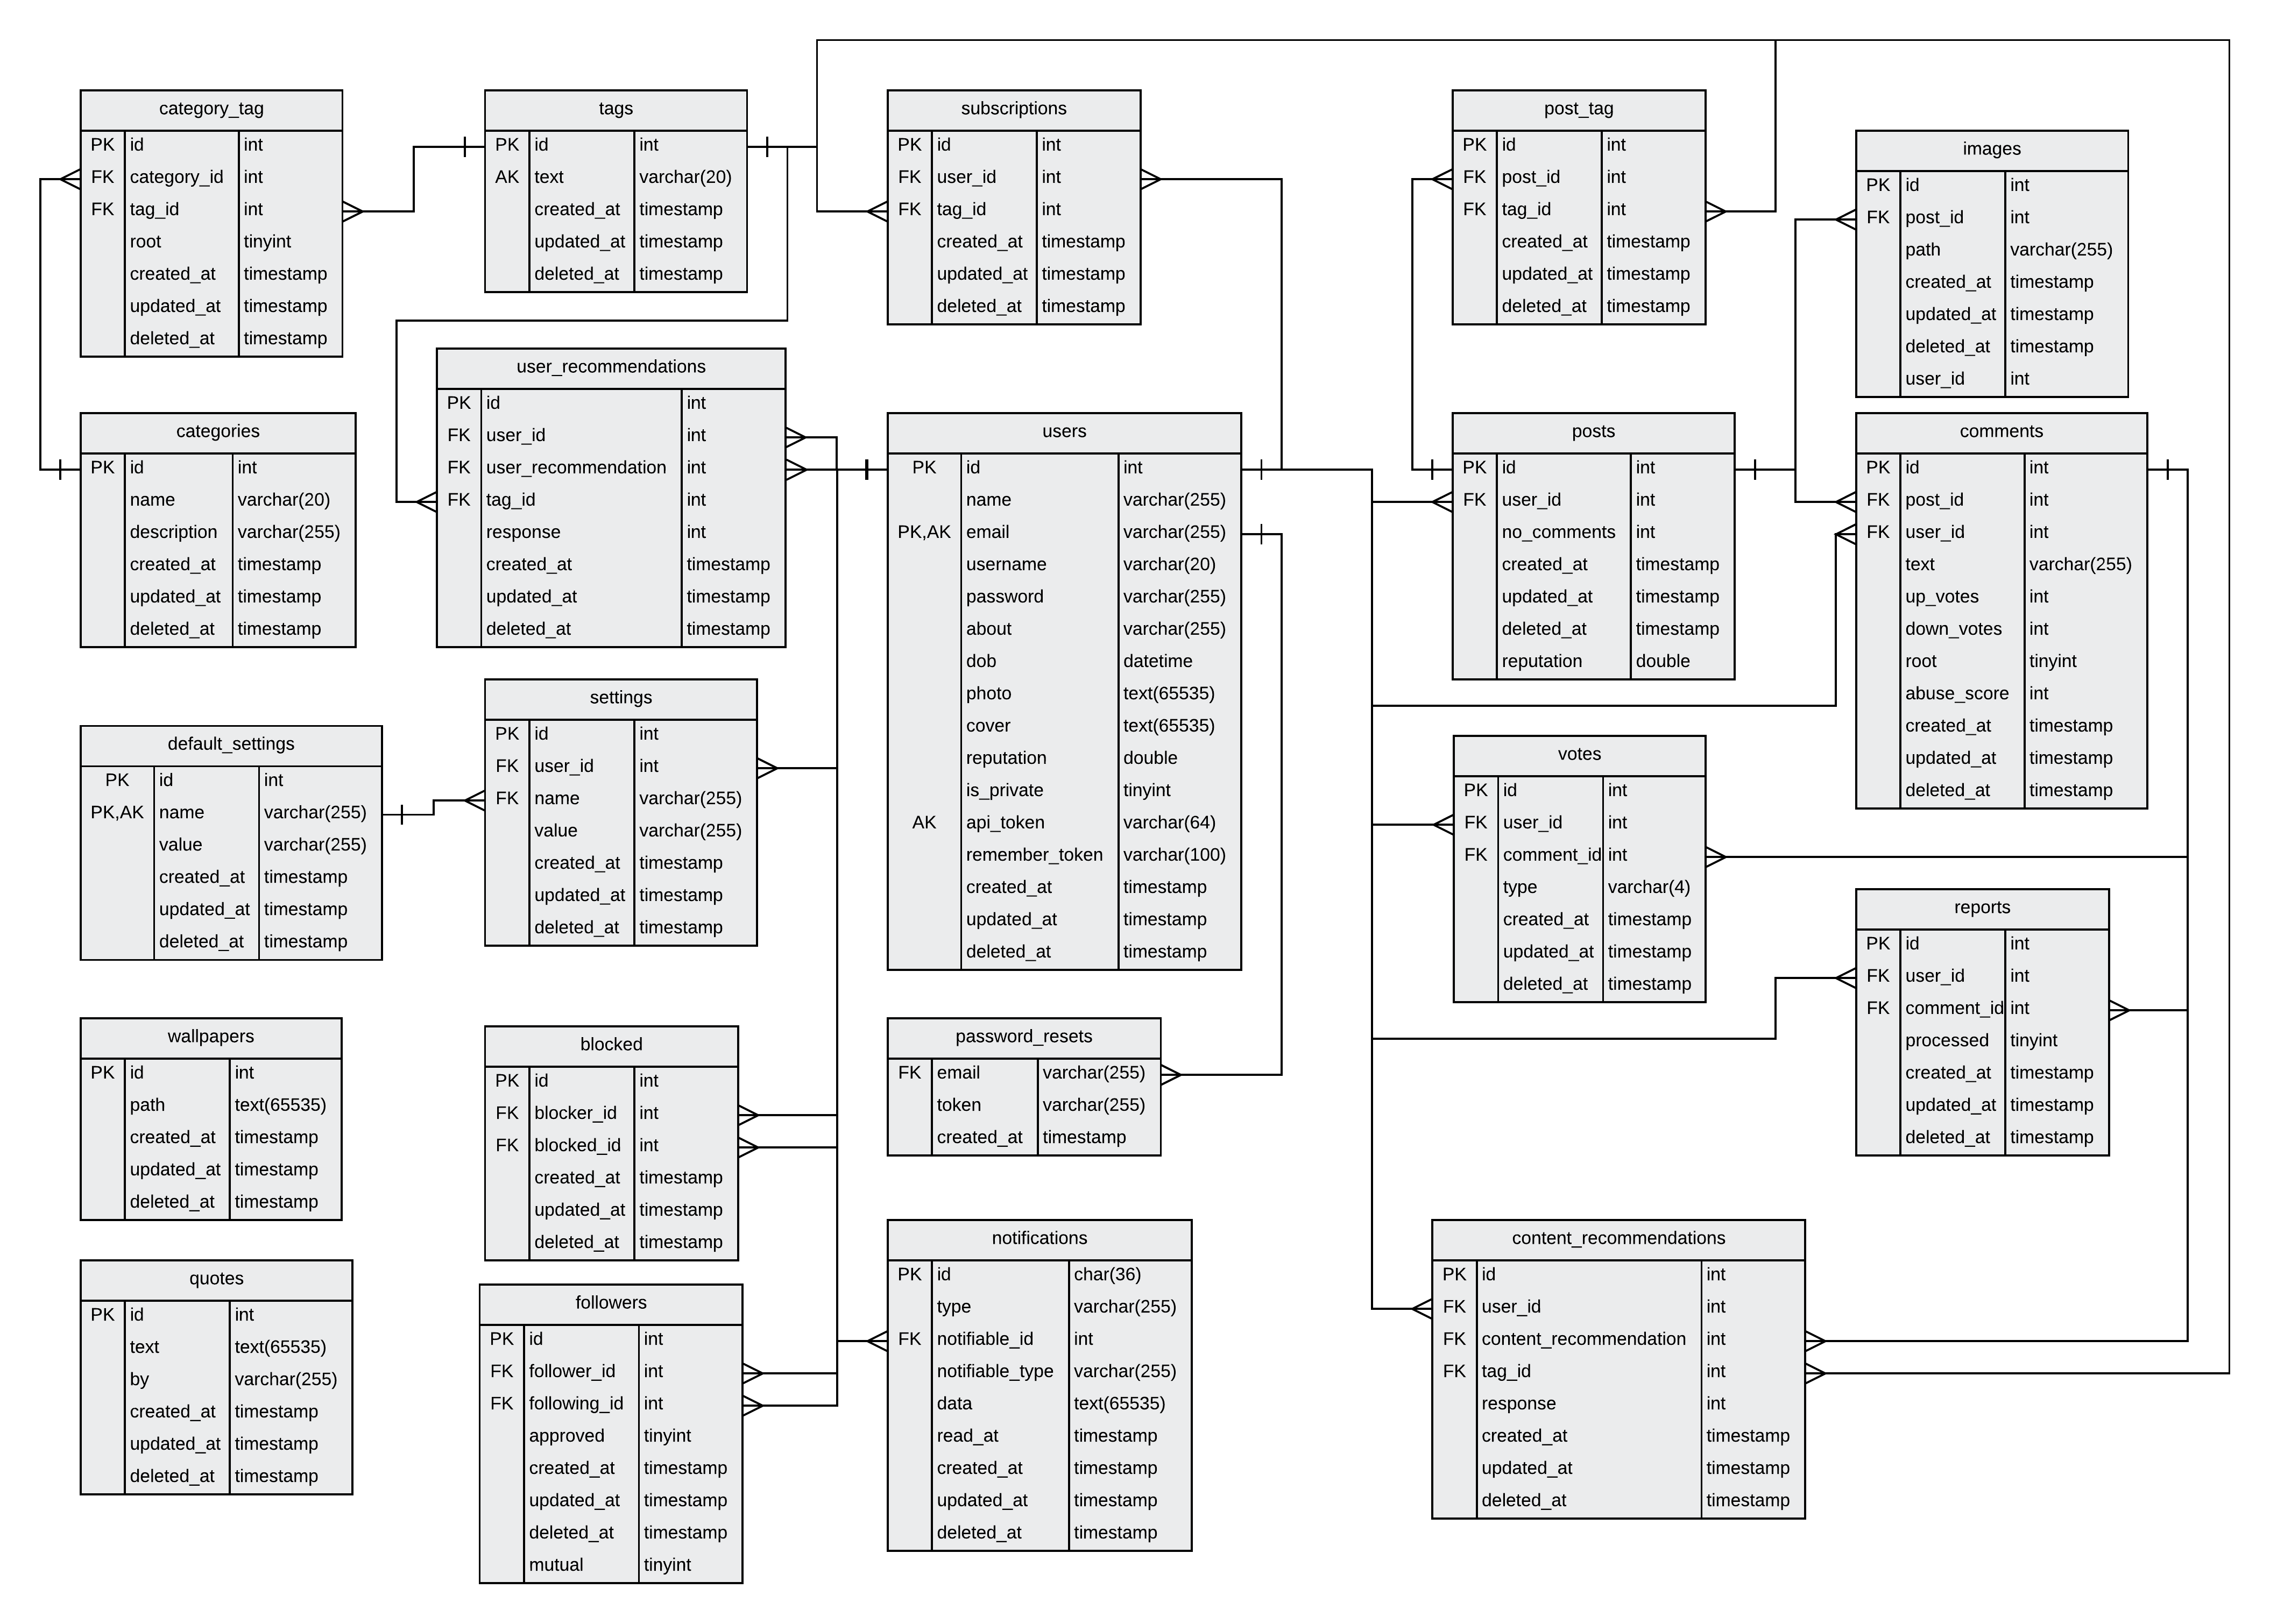
\includegraphics[width=1.0\textwidth]{Images/Design/Database/ERD}
  \caption{Database Schema Represented as an Entity Relationship Diagram (ERD).} \label{fig:Database_ERD}
\end{figure}

\subsection{Tables}
\label{SubSection:Database_Tables}
As mentioned previously, the database consists of many tables comprising many components of the systems. The design of each of the tables, categorised by components, is discussed in this section.

\subsubsection{User and Authentication}
The user is one of the core components of the system. A significant amount of the functionality provided by the system, including but not limited to the authentication system, is reliant upon the user table. This can be seen be the dependencies on the user table in figure \ref{fig:Database_ERD}. Despite the fact that the users details are stored in just one detail, the entire component is comprised of two tables due to the authentication mechanism. The main table which hold the user data is called `users'. Along with its primary key field, id, it also has a primary key on the email field and an alternate key on the email and api token field. This will allow for quick fetching of the user using the api token field when accessing the API. The second table comprising the authentication mechanism is the password resets table which stores recovery tokens when the user makes a forgotten password request. Unlike the other tables, this table does not have an id field but instead it has a foreign key, email, relating a recovery token to the user who requested it. This constraint is also the reason for the index on the email field in the users table.

\subsubsection{Settings}

\subsubsection{Following}

\subsubsection{Categories and Tags}

\subsubsection{Subscriptions}

\subsubsection{Posts and Comments}

\subsubsection{Voting}

\subsubsection{Reporting}

\subsubsection{Notifications}

\subsubsection{Recommendation}

\subsection{Normalisation and Redundancy}
\label{SubSection:Database_Normalisation}

\subsection{Functional Dependencies and Relationship Constraints}
\label{SubSection:Database_Constraints}

\subsection{Security}
\label{SubSection:Database_Security}